\documentclass{report}
\usepackage{fullpage}
\usepackage{hyperref}
\usepackage{graphicx}
\usepackage[margin=0.5in,top=0.5in,bottom=0.5in]{geometry}
\hypersetup{
    colorlinks=true,
    linkcolor=blue,
    filecolor=magenta,
    urlcolor=cyan,
}
\renewcommand{\baselinestretch}{2}
\author{Ahmed Ashraf Abdelkarim - Amr Abdelsamee Yousef - Hazem Abdallah Mohammed}
\title{Visual question answering}
\begin{document}
\maketitle
\tableofcontents
\section{Introduction}
Visual Question Answering (VQA) is the task of answering open-ended questions based on an image. VQA has many applications: Medical VQA, Education purposes, for surveillance and numerous other applications. In this assignment we will use Viz-Wiz data-set, this data-set was constructed to train models to help visually impaired people. In the words of creators of Viz-Wiz: “we introduce the visual question answering (VQA) data-set coming from this population, which we call Viz-Wiz-VQA. It originates from a natural visual question answering setting where blind people each took an image and recorded a spoken question about it, together with 10 crowd sourced answers per visual question.

\section{Data}
\subsection{What is Viz-Wiz?}
The Viz-Wiz data-set is a widely-used benchmark data-set for visual question answering (VQA) tasks. It is designed to evaluate the ability of machine learning models to answer questions about visual content, such as images and videos.

The dataset was created by researchers at the University of Rochester in collaboration with the VizWiz project, which aims to improve access to visual information for people with visual impairments. The dataset contains over 31,000 images, each with a corresponding question and answer pair collected from real-world scenarios.

The Viz-Wiz data-set is unique in that it contains questions and answers that are generated by non-expert users, making it more representative of the types of questions that people might ask in real-world situations. The data-set also includes additional information such as image captions and textual context, which can help models better understand the visual content and answer questions more accurately.

The VizWiz dataset has been used in a variety of research studies and competitions, and has led to significant advances in VQA technology. It remains an important resource for researchers and developers working in this field.

\subsection{How to load the data-set?}
To load data into Google Colab using Kaggle API, follow these steps:

\begin{itemize}
\item Download the Kaggle API credentials from your Kaggle account and upload them to your Google Drive.
\item Install the Kaggle API in your Google Colab notebook.
\item Use the Kaggle API to download data-sets directly to your notebook.
\item Unzip the data
\end{itemize}

That's it! You can now use the downloaded data in your machine learning models on Google Colab.


\subsection{Selecting the best answer}
As stated above each question is supplied with 10 answers along with an answer confidence for each answer. We encoded the confidence as follows:

\begin{itemize}
\item YES maps to 3
\item Maybe maps to 2
\item No maps to 1
\end{itemize}

Then we repeat each answer a number of instances equivalent to the confidence encoded value. Then if there is only 1 answer repeated maximum number of times then it is the chosen answer for this question. In case 2 or more are repeated equally we check which one of them is repeated maximum number of times in the data-set to check if the answer is not an out-liner and if more than one is equal we use the \href{https://medium.com/@ethannam/understanding-the-levenshtein-distance-equation-for-beginners-c4285a5604f0#:~:text=The%20Levenshtein%20distance%20is%20a,change%20one%20into%20the%20other.}{\textbf{Levenshtein distance}} to see which one is more representative of the data
\subsection{Random samples visualisation}
Here are some random samples along with their questions and other data visualized:\\
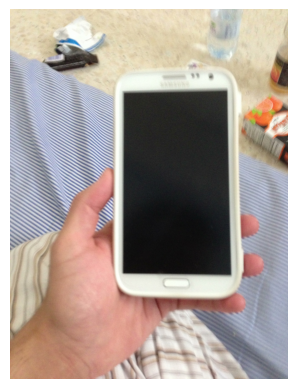
\includegraphics[width=0.5\linewidth]{phone.png}\\
questions : What  Is this?\\
answerable :1\\
answer type :other\\
answers:[android phone, cell phone, cell phone, cellphone, samsung phone, unanswerable, phone, smart phone, white smartphone, phone]\\
answer confidence[maybe, maybe, maybe, maybe, yes, yes, yes, yes, yes, yes]  \\                                                     

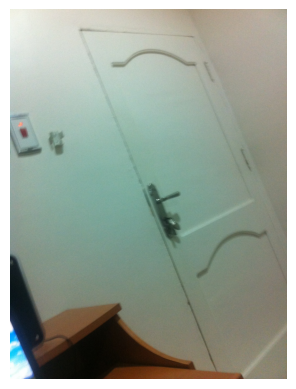
\includegraphics[width=0.5\linewidth]{door.png}\\
questions:Oh, what's this?\\
answerable:1\\
answer type:other\\
answers:[unanswerable, door, door, door locks, door, door, door, door, door, door]\\
answer confidence:[yes, yes, yes, yes, yes, yes, yes, yes, yes, maybe]\\


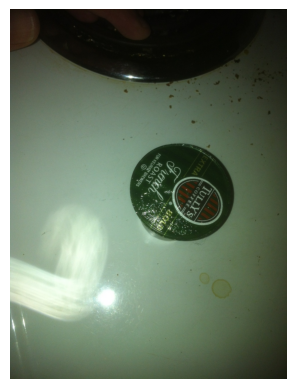
\includegraphics[width=0.5\linewidth]{toast.png}\\
questions:What flavor and make of coffee is this, please?\\
answerable:1\\
answer type:other\\
answers:[french roast tullys, tullys french roast, tullys french roast, tolls, unanswerable, unsuitable, french roast, tullys french roast, unsuitable, tullys french roast]\\
answer confidence:[yes, yes, yes, maybe, no, yes, maybe, yes, yes, yes]\\

    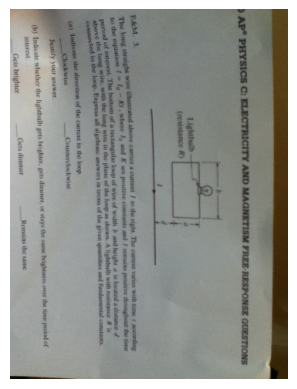
\includegraphics[width=0.5\linewidth]{paper.png}\\
questions: What is the direction of the curtain loop and why?\\
answerable:0\\
answer type:unanswerable\\
answers:[unanswerable, unanswerable, unanswerable, unanswerable, unanswerable, unanswerable, unanswerable, unanswerable, unanswerable, unanswerable]\\
answer confidence:[no, no, yes, yes, yes, yes, no, yes, yes, yes]

\subsection{Some finer details about the data}
Some questions are repeated many times in the model as shown in the histogram below\\
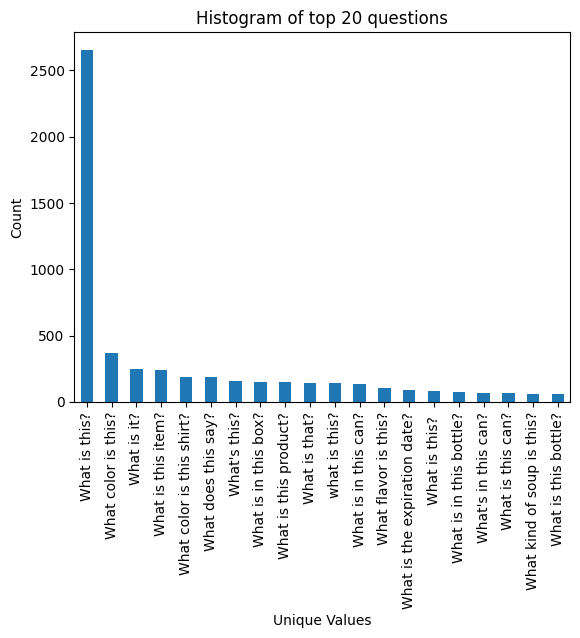
\includegraphics[width=0.5\textwidth]{top20questions.png}\\
Also some answers are repeated more than others as shown in the histogram below\\
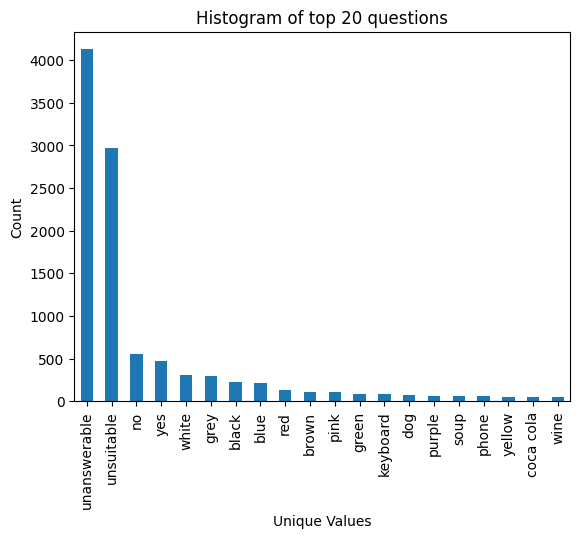
\includegraphics[width=0.5\textwidth]{top20answers.png}
\\\\\\\\\\Also shown below the top 20 answer types\\
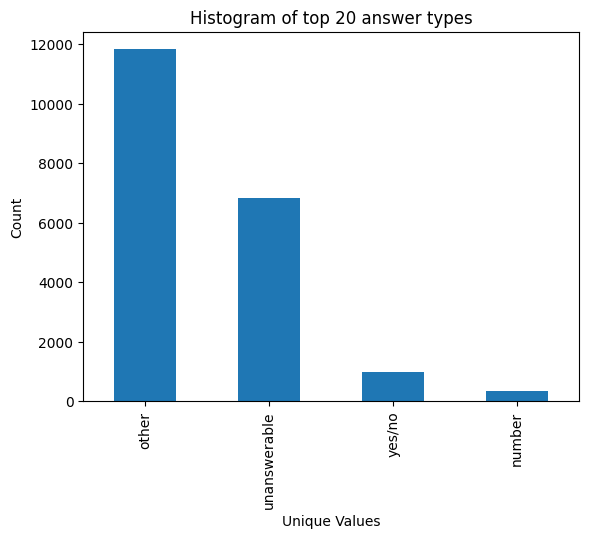
\includegraphics[width=0.5\linewidth]{toptypes.png}
\\And also shown the count of answerable vs unanswerable questions\\
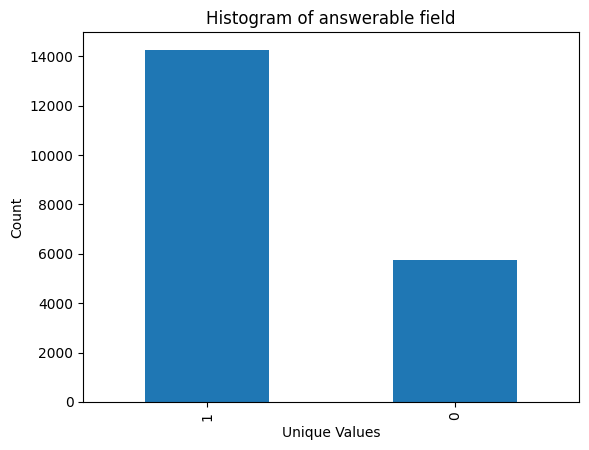
\includegraphics[width=0.5\linewidth]{ans.png}\\
The last step before applying the data to our model was to encode the answers and answer types using one hot encoding



\section{Model}
We will discuss here each part of the code in a seprate subsection
\subsection{VQA model class}
This code defines a PyTorch neural network model for visual question answering (VQA). The model takes as input an image and a question, and outputs a predicted answer to the question.

The VQAModel class inherits from the nn.Module class, which is the base class for all neural network modules in PyTorch. In the init method, the model defines its layers and parameters.

The forward method defines the forward pass of the model, which computes the output given the input. The input consists of an image tensor and a question tensor, which are concatenated along the feature dimension using the torch.cat method. The concatenated features are then passed through a linear layer with 512 output units, followed by a layer normalization, ReLU activation, and dropout. The output of this layer is then passed through another linear layer with num classes output units, which corresponds to the number of possible answers in the dataset. The output is then returned as the predicted answer.

Overall, this code provides a basic template for building a VQA model using PyTorch.

\subsection{VQA dataset class}
This is a PyTorch dataset class for the visual question answering (VQA) task. The VQADataset class inherits from the Dataset class in PyTorch, which is the base class for all datasets in PyTorch.

In the init method, the class initializes the dataset by taking in the image names, questions, answers, answer types, tokenizer, and transform. These arguments are stored as attributes of the class for later use. Additionally, the method loads the CLIP model using the clip.load method and stores it as an attribute of the class.

The len method returns the length of the dataset, which is the number of images in the dataset.

The getitem method defines how to retrieve an item from the dataset given an index. The method first retrieves the answer and answer type corresponding to the given index. It then reads and transforms the image using the PIL library, encodes the image using the CLIP model, and retrieves the image features. Next, it tokenizes the question using the given tokenizer, encodes the question using the CLIP model, and retrieves the question features. Finally, it returns the image features, question features, answer, and answer type as a tuple.

Overall, this class provides a data pipeline for preparing the input data for a VQA model using PyTorch.

\subsection{data training}
The data train procedure is done as follows:\\
Initialize some variables to keep track of the totalloss and accuracy for the answers and answer types.\\
Set the model to training mode using model.train().\\
Loop through each batch of data in the data loader.\\
Move the data to the device (e.g. GPU) specified in the device variable.\\
Zero out the gradients in the optimizer using optimizer.zerograd().\\
Pass the encoded data through the model using output, aux = model(encoded data), which returns the model's output for both the answer and answer type.\\
Squeeze the output tensors to remove any extra dimensions using torch.squeeze().\\
Compute the answer loss and answer type loss separately using loss.fn(output, answers) and loss.fn(aux, answers types), respectively.\\
Compute the total loss as the sum of the answer loss and answer type loss.\\
Back propagate the total loss through the model using loss.backward().\\
Update the model's parameters using the optimizer with optimizer.step().\\
Calculate the accuracy for the answers by comparing the model's predicted answer to the true answer using (predicted = answers).sum().item().\\
Calculate the accuracy for the answer types in the same way.\\
Calculate the total accuracy as the average of the answer accuracy and answer type accuracy.\\
Calculate the total loss as the average of the per-batch loss.\\
Return the total loss, total accuracy, answer accuracy, and answer type accuracy.\\

\subsection{Model eval}
The model evaluation is done as follows:\\
Initialize some variables to keep track of the total loss and accuracy for the answers and answer types.\\
Set the model to evaluation mode using model.eval().\\
Disable gradient calculation using with torch.nograd(): to speed up evaluation and save memory.\\
Loop through each batch of data in the dataloader.\\
Move the data to the device (e.g. GPU) specified in the device variable.\\
Pass the encoded data through the model using output, aux = model(encodeddata), which returns the model's output for both the answer and answer type.\\
Squeeze the output tensors to remove any extra dimensions using torch.squeeze().\\
Compute the answer loss and answer type loss separately using lossfn(output, answers) and lossfn(aux, answerstypes), respectively.\\
Compute the total loss as the sum of the answer loss and answer type loss.\\
Calculate the accuracy for the answers by comparing the model's predicted answer to the true answer using (predicted == answers).sum().item().\\
Calculate the accuracy for the answer types in the same way as step 10.\\
Calculate the total accuracy as the average of the answer accuracy and answer type accuracy.\\
Calculate the total loss as the average of the per-batch loss.\\
Return the total loss, total accuracy, answer accuracy, and answer type accuracy.\\

\subsection{Predictions}
The prediction procdeure is done as follows:
Disable gradient calculation using with torch.nograd(): to speed up prediction and save memory.\\
Pass the encoded data through the model using output, aux = model(encodeddata), which returns the model's output for both the answer and answer type.\\
Squeeze the output tensors to remove any extra dimensions using torch.squeeze().\\
Compute the predicted answer by finding the index of the maximum value in output using torch.max(output.data, 1).\\
Compute the predicted answer type in the same way as step 4 but using aux instead of output.\\
Decode the predicted answer and answer type using the respective inverse transformers answersencoder.inversetransform() and answerstypesencoder.inversetransform().\\
Return the predicted answer and answer type as strings.\\

\section{Results}
\subsection{Training results}
\begin{verbatim}
Epoch: 1/80 - Learning Rate:  0.001000
 loss:  0.9367 - accuracy:  0.8192 - val-loss:  22.4993 - val-accuracy:  0.3422
 ans-acc:  0.8005 - ans-type-acc:  0.8380 - val-ans-acc:  0.0000 - val-ans-type-acc:  0.6844
------------------------------------
Epoch: 2/80 - Learning Rate:  0.001000
 loss:  0.9212 - accuracy:  0.8232 - val-loss:  22.0382 - val-accuracy:  0.3360
 ans-acc:  0.8052 - ans-type-acc:  0.8412 - val-ans-acc:  0.0000 - val-ans-type-acc:  0.6719
------------------------------------
Epoch: 3/80 - Learning Rate:  0.001000
 loss:  0.9389 - accuracy:  0.8187 - val-loss:  22.6154 - val-accuracy:  0.3512
 ans-acc:  0.8015 - ans-type-acc:  0.8359 - val-ans-acc:  0.0000 - val-ans-type-acc:  0.7025
------------------------------------
Epoch: 4/80 - Learning Rate:  0.001000
 loss:  0.9399 - accuracy:  0.8201 - val-loss:  22.1885 - val-accuracy:  0.3479
 ans-acc:  0.8024 - ans-type-acc:  0.8378 - val-ans-acc:  0.0000 - val-ans-type-acc:  0.6958
------------------------------------
Epoch: 5/80 - Learning Rate:  0.001000
 loss:  0.9271 - accuracy:  0.8195 - val-loss:  22.1841 - val-accuracy:  0.3427
 ans-acc:  0.8014 - ans-type-acc:  0.8376 - val-ans-acc:  0.0000 - val-ans-type-acc:  0.6853
------------------------------------
Epoch: 6/80 - Learning Rate:  0.001000
 loss:  0.9307 - accuracy:  0.8204 - val-loss:  22.1402 - val-accuracy:  0.3493
 ans-acc:  0.8037 - ans-type-acc:  0.8370 - val-ans-acc:  0.0000 - val-ans-type-acc:  0.6985
------------------------------------
Epoch: 7/80 - Learning Rate:  0.001000
 loss:  0.9338 - accuracy:  0.8202 - val-loss:  22.3786 - val-accuracy:  0.3494
 ans-acc:  0.8053 - ans-type-acc:  0.8350 - val-ans-acc:  0.0000 - val-ans-type-acc:  0.6988
------------------------------------
Epoch: 8/80 - Learning Rate:  0.001000
 loss:  0.9367 - accuracy:  0.8201 - val-loss:  22.0682 - val-accuracy:  0.3433
 ans-acc:  0.8022 - ans-type-acc:  0.8380 - val-ans-acc:  0.0000 - val-ans-type-acc:  0.6865
------------------------------------
Epoch: 9/80 - Learning Rate:  0.001000
 loss:  0.9357 - accuracy:  0.8173 - val-loss:  22.4710 - val-accuracy:  0.3455
 ans-acc:  0.7999 - ans-type-acc:  0.8348 - val-ans-acc:  0.0000 - val-ans-type-acc:  0.6909
------------------------------------
Epoch: 10/80 - Learning Rate:  0.001000
 loss:  0.9251 - accuracy:  0.8223 - val-loss:  22.2413 - val-accuracy:  0.3540
 ans-acc:  0.8042 - ans-type-acc:  0.8405 - val-ans-acc:  0.0000 - val-ans-type-acc:  0.7080
------------------------------------
Epoch: 11/80 - Learning Rate:  0.001000
 loss:  0.9246 - accuracy:  0.8216 - val-loss:  22.4299 - val-accuracy:  0.3518
 ans-acc:  0.8042 - ans-type-acc:  0.8390 - val-ans-acc:  0.0000 - val-ans-type-acc:  0.7036
------------------------------------
Epoch: 12/80 - Learning Rate:  0.001000
 loss:  0.9222 - accuracy:  0.8227 - val-loss:  22.3014 - val-accuracy:  0.3389
 ans-acc:  0.8035 - ans-type-acc:  0.8419 - val-ans-acc:  0.0000 - val-ans-type-acc:  0.6777
------------------------------------
Epoch: 13/80 - Learning Rate:  0.001000
 loss:  0.9394 - accuracy:  0.8189 - val-loss:  22.1078 - val-accuracy:  0.3402
 ans-acc:  0.7969 - ans-type-acc:  0.8409 - val-ans-acc:  0.0000 - val-ans-type-acc:  0.6805
------------------------------------
Epoch: 14/80 - Learning Rate:  0.001000
 loss:  0.9351 - accuracy:  0.8216 - val-loss:  22.4214 - val-accuracy:  0.3568
 ans-acc:  0.8045 - ans-type-acc:  0.8386 - val-ans-acc:  0.0000 - val-ans-type-acc:  0.7136
------------------------------------
Epoch: 15/80 - Learning Rate:  0.001000
 loss:  0.9344 - accuracy:  0.8207 - val-loss:  22.1878 - val-accuracy:  0.3514
 ans-acc:  0.8009 - ans-type-acc:  0.8404 - val-ans-acc:  0.0000 - val-ans-type-acc:  0.7027
------------------------------------
Epoch: 16/80 - Learning Rate:  0.001000
 loss:  0.9261 - accuracy:  0.8223 - val-loss:  22.0804 - val-accuracy:  0.3457
 ans-acc:  0.8008 - ans-type-acc:  0.8438 - val-ans-acc:  0.0000 - val-ans-type-acc:  0.6914
------------------------------------
Epoch: 17/80 - Learning Rate:  0.001000
 loss:  0.9362 - accuracy:  0.8190 - val-loss:  22.2413 - val-accuracy:  0.3460
 ans-acc:  0.8003 - ans-type-acc:  0.8378 - val-ans-acc:  0.0000 - val-ans-type-acc:  0.6921
------------------------------------
Epoch: 18/80 - Learning Rate:  0.001000
 loss:  0.9185 - accuracy:  0.8238 - val-loss:  22.2664 - val-accuracy:  0.3424
 ans-acc:  0.8055 - ans-type-acc:  0.8421 - val-ans-acc:  0.0000 - val-ans-type-acc:  0.6849
------------------------------------
Epoch: 19/80 - Learning Rate:  0.001000
 loss:  0.9259 - accuracy:  0.8226 - val-loss:  22.1927 - val-accuracy:  0.3443
 ans-acc:  0.8039 - ans-type-acc:  0.8412 - val-ans-acc:  0.0000 - val-ans-type-acc:  0.6886
------------------------------------
Epoch: 20/80 - Learning Rate:  0.001000
 loss:  0.9310 - accuracy:  0.8221 - val-loss:  22.1547 - val-accuracy:  0.3569
 ans-acc:  0.8039 - ans-type-acc:  0.8403 - val-ans-acc:  0.0000 - val-ans-type-acc:  0.7138
------------------------------------
Epoch: 21/80 - Learning Rate:  0.001000
 loss:  0.9295 - accuracy:  0.8211 - val-loss:  22.3620 - val-accuracy:  0.3369
 ans-acc:  0.8018 - ans-type-acc:  0.8405 - val-ans-acc:  0.0000 - val-ans-type-acc:  0.6738
------------------------------------
Epoch: 22/80 - Learning Rate:  0.001000
 loss:  0.9293 - accuracy:  0.8230 - val-loss:  22.4011 - val-accuracy:  0.3402
 ans-acc:  0.8092 - ans-type-acc:  0.8367 - val-ans-acc:  0.0000 - val-ans-type-acc:  0.6805
------------------------------------
Epoch: 23/80 - Learning Rate:  0.001000
 loss:  0.9200 - accuracy:  0.8224 - val-loss:  22.5403 - val-accuracy:  0.3257
 ans-acc:  0.8018 - ans-type-acc:  0.8430 - val-ans-acc:  0.0000 - val-ans-type-acc:  0.6513
------------------------------------
Epoch: 24/80 - Learning Rate:  0.001000
 loss:  0.9247 - accuracy:  0.8225 - val-loss:  22.5837 - val-accuracy:  0.3397
 ans-acc:  0.8014 - ans-type-acc:  0.8436 - val-ans-acc:  0.0000 - val-ans-type-acc:  0.6793
------------------------------------
Epoch: 25/80 - Learning Rate:  0.001000
 loss:  0.9301 - accuracy:  0.8218 - val-loss:  22.5083 - val-accuracy:  0.3431
 ans-acc:  0.8013 - ans-type-acc:  0.8422 - val-ans-acc:  0.0000 - val-ans-type-acc:  0.6863
------------------------------------
Epoch: 26/80 - Learning Rate:  0.001000
 loss:  0.9274 - accuracy:  0.8236 - val-loss:  21.9544 - val-accuracy:  0.3419
 ans-acc:  0.8007 - ans-type-acc:  0.8464 - val-ans-acc:  0.0000 - val-ans-type-acc:  0.6837
------------------------------------
Epoch: 27/80 - Learning Rate:  0.001000
 loss:  0.9272 - accuracy:  0.8216 - val-loss:  22.1667 - val-accuracy:  0.3461
 ans-acc:  0.8019 - ans-type-acc:  0.8412 - val-ans-acc:  0.0000 - val-ans-type-acc:  0.6923
------------------------------------
Epoch: 28/80 - Learning Rate:  0.001000
 loss:  0.9291 - accuracy:  0.8212 - val-loss:  22.3193 - val-accuracy:  0.3395
 ans-acc:  0.8006 - ans-type-acc:  0.8419 - val-ans-acc:  0.0000 - val-ans-type-acc:  0.6791
------------------------------------
Epoch: 29/80 - Learning Rate:  0.001000
 loss:  0.9254 - accuracy:  0.8201 - val-loss:  22.5868 - val-accuracy:  0.3342
 ans-acc:  0.8022 - ans-type-acc:  0.8380 - val-ans-acc:  0.0000 - val-ans-type-acc:  0.6684
------------------------------------
Epoch: 30/80 - Learning Rate:  0.001000
 loss:  0.9351 - accuracy:  0.8215 - val-loss:  22.4855 - val-accuracy:  0.3497
 ans-acc:  0.7997 - ans-type-acc:  0.8433 - val-ans-acc:  0.0000 - val-ans-type-acc:  0.6995
------------------------------------
Epoch: 31/80 - Learning Rate:  0.001000
 loss:  0.9351 - accuracy:  0.8209 - val-loss:  22.1960 - val-accuracy:  0.3437
 ans-acc:  0.8006 - ans-type-acc:  0.8412 - val-ans-acc:  0.0000 - val-ans-type-acc:  0.6874
------------------------------------
Epoch: 32/80 - Learning Rate:  0.001000
 loss:  0.9292 - accuracy:  0.8191 - val-loss:  22.4734 - val-accuracy:  0.3422
 ans-acc:  0.7986 - ans-type-acc:  0.8396 - val-ans-acc:  0.0000 - val-ans-type-acc:  0.6844
------------------------------------
Epoch: 33/80 - Learning Rate:  0.001000
 loss:  0.9204 - accuracy:  0.8240 - val-loss:  22.2466 - val-accuracy:  0.3455
 ans-acc:  0.8048 - ans-type-acc:  0.8431 - val-ans-acc:  0.0000 - val-ans-type-acc:  0.6909
------------------------------------
Epoch: 34/80 - Learning Rate:  0.001000
 loss:  0.9205 - accuracy:  0.8229 - val-loss:  22.2687 - val-accuracy:  0.3461
 ans-acc:  0.8032 - ans-type-acc:  0.8426 - val-ans-acc:  0.0000 - val-ans-type-acc:  0.6923
------------------------------------
Epoch: 35/80 - Learning Rate:  0.001000
 loss:  0.9201 - accuracy:  0.8213 - val-loss:  22.3835 - val-accuracy:  0.3391
 ans-acc:  0.7990 - ans-type-acc:  0.8435 - val-ans-acc:  0.0000 - val-ans-type-acc:  0.6782
------------------------------------
Epoch: 36/80 - Learning Rate:  0.001000
 loss:  0.9224 - accuracy:  0.8236 - val-loss:  22.2201 - val-accuracy:  0.3487
 ans-acc:  0.8051 - ans-type-acc:  0.8421 - val-ans-acc:  0.0000 - val-ans-type-acc:  0.6974
------------------------------------
Epoch: 37/80 - Learning Rate:  0.001000
 loss:  0.9250 - accuracy:  0.8229 - val-loss:  22.2426 - val-accuracy:  0.3445
 ans-acc:  0.8029 - ans-type-acc:  0.8428 - val-ans-acc:  0.0000 - val-ans-type-acc:  0.6890
------------------------------------
Epoch: 38/80 - Learning Rate:  0.001000
 loss:  0.9285 - accuracy:  0.8205 - val-loss:  22.0677 - val-accuracy:  0.3471
 ans-acc:  0.7993 - ans-type-acc:  0.8417 - val-ans-acc:  0.0000 - val-ans-type-acc:  0.6941
------------------------------------
Epoch: 39/80 - Learning Rate:  0.001000
 loss:  0.9320 - accuracy:  0.8227 - val-loss:  22.2687 - val-accuracy:  0.3437
 ans-acc:  0.7991 - ans-type-acc:  0.8462 - val-ans-acc:  0.0000 - val-ans-type-acc:  0.6874
------------------------------------
Epoch: 40/80 - Learning Rate:  0.001000
 loss:  0.9325 - accuracy:  0.8202 - val-loss:  22.0783 - val-accuracy:  0.3298
 ans-acc:  0.8010 - ans-type-acc:  0.8394 - val-ans-acc:  0.0000 - val-ans-type-acc:  0.6596
------------------------------------
Epoch: 41/80 - Learning Rate:  0.001000
 loss:  0.9208 - accuracy:  0.8239 - val-loss:  22.0661 - val-accuracy:  0.3430
 ans-acc:  0.8030 - ans-type-acc:  0.8447 - val-ans-acc:  0.0000 - val-ans-type-acc:  0.6860
------------------------------------
Epoch: 42/80 - Learning Rate:  0.001000
 loss:  0.9193 - accuracy:  0.8235 - val-loss:  22.5554 - val-accuracy:  0.3340
 ans-acc:  0.8048 - ans-type-acc:  0.8422 - val-ans-acc:  0.0000 - val-ans-type-acc:  0.6680
------------------------------------
Epoch: 43/80 - Learning Rate:  0.001000
 loss:  0.9149 - accuracy:  0.8254 - val-loss:  22.4360 - val-accuracy:  0.3424
 ans-acc:  0.8043 - ans-type-acc:  0.8466 - val-ans-acc:  0.0000 - val-ans-type-acc:  0.6849
------------------------------------
Epoch: 44/80 - Learning Rate:  0.001000
 loss:  0.9206 - accuracy:  0.8256 - val-loss:  22.1485 - val-accuracy:  0.3407
 ans-acc:  0.8043 - ans-type-acc:  0.8468 - val-ans-acc:  0.0000 - val-ans-type-acc:  0.6814
------------------------------------
Epoch: 45/80 - Learning Rate:  0.001000
 loss:  0.9216 - accuracy:  0.8217 - val-loss:  22.3442 - val-accuracy:  0.3376
 ans-acc:  0.8003 - ans-type-acc:  0.8430 - val-ans-acc:  0.0000 - val-ans-type-acc:  0.6752
------------------------------------
Epoch: 46/80 - Learning Rate:  0.001000
 loss:  0.9185 - accuracy:  0.8227 - val-loss:  22.1014 - val-accuracy:  0.3420
 ans-acc:  0.8025 - ans-type-acc:  0.8429 - val-ans-acc:  0.0000 - val-ans-type-acc:  0.6840
------------------------------------
Epoch: 47/80 - Learning Rate:  0.001000
 loss:  0.9254 - accuracy:  0.8227 - val-loss:  22.2772 - val-accuracy:  0.3347
 ans-acc:  0.8032 - ans-type-acc:  0.8423 - val-ans-acc:  0.0000 - val-ans-type-acc:  0.6694
------------------------------------
Epoch: 48/80 - Learning Rate:  0.001000
 loss:  0.9132 - accuracy:  0.8249 - val-loss:  22.3271 - val-accuracy:  0.3417
 ans-acc:  0.8062 - ans-type-acc:  0.8436 - val-ans-acc:  0.0000 - val-ans-type-acc:  0.6835
------------------------------------
Epoch: 49/80 - Learning Rate:  0.001000
 loss:  0.9272 - accuracy:  0.8230 - val-loss:  22.3893 - val-accuracy:  0.3426
 ans-acc:  0.8012 - ans-type-acc:  0.8448 - val-ans-acc:  0.0000 - val-ans-type-acc:  0.6851
------------------------------------
Epoch: 50/80 - Learning Rate:  0.001000
 loss:  0.9102 - accuracy:  0.8256 - val-loss:  22.3156 - val-accuracy:  0.3393
 ans-acc:  0.8013 - ans-type-acc:  0.8498 - val-ans-acc:  0.0000 - val-ans-type-acc:  0.6786
------------------------------------
Epoch: 51/80 - Learning Rate:  0.001000
 loss:  0.9161 - accuracy:  0.8262 - val-loss:  22.3836 - val-accuracy:  0.3329
 ans-acc:  0.8059 - ans-type-acc:  0.8465 - val-ans-acc:  0.0000 - val-ans-type-acc:  0.6659
------------------------------------
Epoch: 52/80 - Learning Rate:  0.001000
 loss:  0.9206 - accuracy:  0.8227 - val-loss:  22.5466 - val-accuracy:  0.3444
 ans-acc:  0.8005 - ans-type-acc:  0.8449 - val-ans-acc:  0.0000 - val-ans-type-acc:  0.6888
------------------------------------
Epoch: 53/80 - Learning Rate:  0.001000
 loss:  0.9201 - accuracy:  0.8242 - val-loss:  22.3606 - val-accuracy:  0.3479
 ans-acc:  0.8024 - ans-type-acc:  0.8459 - val-ans-acc:  0.0000 - val-ans-type-acc:  0.6958
------------------------------------
Epoch: 54/80 - Learning Rate:  0.001000
 loss:  0.9115 - accuracy:  0.8256 - val-loss:  22.4209 - val-accuracy:  0.3316
 ans-acc:  0.8028 - ans-type-acc:  0.8484 - val-ans-acc:  0.0000 - val-ans-type-acc:  0.6631
------------------------------------
Epoch: 55/80 - Learning Rate:  0.001000
 loss:  0.9214 - accuracy:  0.8227 - val-loss:  22.4022 - val-accuracy:  0.3420
 ans-acc:  0.8018 - ans-type-acc:  0.8435 - val-ans-acc:  0.0000 - val-ans-type-acc:  0.6840
------------------------------------
Epoch: 56/80 - Learning Rate:  0.001000
 loss:  0.9232 - accuracy:  0.8218 - val-loss:  22.3166 - val-accuracy:  0.3354
 ans-acc:  0.7989 - ans-type-acc:  0.8447 - val-ans-acc:  0.0000 - val-ans-type-acc:  0.6708
------------------------------------
Epoch: 57/80 - Learning Rate:  0.001000
 loss:  0.9243 - accuracy:  0.8224 - val-loss:  22.1637 - val-accuracy:  0.3296
 ans-acc:  0.8007 - ans-type-acc:  0.8442 - val-ans-acc:  0.0000 - val-ans-type-acc:  0.6592
------------------------------------
Epoch: 58/80 - Learning Rate:  0.001000
 loss:  0.9280 - accuracy:  0.8207 - val-loss:  22.3258 - val-accuracy:  0.3442
 ans-acc:  0.7982 - ans-type-acc:  0.8432 - val-ans-acc:  0.0000 - val-ans-type-acc:  0.6884
------------------------------------
Epoch: 59/80 - Learning Rate:  0.001000
 loss:  0.9116 - accuracy:  0.8243 - val-loss:  22.1274 - val-accuracy:  0.3365
 ans-acc:  0.8017 - ans-type-acc:  0.8469 - val-ans-acc:  0.0000 - val-ans-type-acc:  0.6731
------------------------------------
Epoch: 60/80 - Learning Rate:  0.001000
 loss:  0.9132 - accuracy:  0.8241 - val-loss:  22.2085 - val-accuracy:  0.3334
 ans-acc:  0.8032 - ans-type-acc:  0.8449 - val-ans-acc:  0.0000 - val-ans-type-acc:  0.6668
------------------------------------
Epoch: 61/80 - Learning Rate:  0.001000
 loss:  0.9119 - accuracy:  0.8252 - val-loss:  22.1241 - val-accuracy:  0.3464
 ans-acc:  0.8054 - ans-type-acc:  0.8449 - val-ans-acc:  0.0000 - val-ans-type-acc:  0.6928
------------------------------------
Epoch: 62/80 - Learning Rate:  0.001000
 loss:  0.9158 - accuracy:  0.8242 - val-loss:  22.1471 - val-accuracy:  0.3402
 ans-acc:  0.8032 - ans-type-acc:  0.8451 - val-ans-acc:  0.0000 - val-ans-type-acc:  0.6805
------------------------------------
Epoch: 63/80 - Learning Rate:  0.001000
 loss:  0.9160 - accuracy:  0.8225 - val-loss:  21.9564 - val-accuracy:  0.3215
 ans-acc:  0.7996 - ans-type-acc:  0.8453 - val-ans-acc:  0.0000 - val-ans-type-acc:  0.6430
------------------------------------
Epoch: 64/80 - Learning Rate:  0.001000
 loss:  0.9211 - accuracy:  0.8246 - val-loss:  22.1525 - val-accuracy:  0.3417
 ans-acc:  0.8000 - ans-type-acc:  0.8491 - val-ans-acc:  0.0000 - val-ans-type-acc:  0.6835
------------------------------------
Epoch: 65/80 - Learning Rate:  0.001000
 loss:  0.9233 - accuracy:  0.8225 - val-loss:  22.1750 - val-accuracy:  0.3475
 ans-acc:  0.7984 - ans-type-acc:  0.8467 - val-ans-acc:  0.0000 - val-ans-type-acc:  0.6951
------------------------------------
Epoch: 66/80 - Learning Rate:  0.001000
 loss:  0.9164 - accuracy:  0.8246 - val-loss:  22.4602 - val-accuracy:  0.3407
 ans-acc:  0.8011 - ans-type-acc:  0.8481 - val-ans-acc:  0.0000 - val-ans-type-acc:  0.6814
------------------------------------
Epoch: 67/80 - Learning Rate:  0.001000
 loss:  0.9145 - accuracy:  0.8262 - val-loss:  22.2900 - val-accuracy:  0.3246
 ans-acc:  0.8065 - ans-type-acc:  0.8460 - val-ans-acc:  0.0000 - val-ans-type-acc:  0.6492
------------------------------------
Epoch: 68/80 - Learning Rate:  0.001000
 loss:  0.9241 - accuracy:  0.8230 - val-loss:  22.4838 - val-accuracy:  0.3390
 ans-acc:  0.8007 - ans-type-acc:  0.8454 - val-ans-acc:  0.0000 - val-ans-type-acc:  0.6779
------------------------------------
Epoch: 69/80 - Learning Rate:  0.001000
 loss:  0.9122 - accuracy:  0.8251 - val-loss:  22.6541 - val-accuracy:  0.3356
 ans-acc:  0.8037 - ans-type-acc:  0.8466 - val-ans-acc:  0.0000 - val-ans-type-acc:  0.6712
------------------------------------
Epoch: 70/80 - Learning Rate:  0.001000
 loss:  0.9178 - accuracy:  0.8250 - val-loss:  22.0941 - val-accuracy:  0.3439
 ans-acc:  0.8040 - ans-type-acc:  0.8460 - val-ans-acc:  0.0000 - val-ans-type-acc:  0.6879
------------------------------------
Epoch: 71/80 - Learning Rate:  0.001000
 loss:  0.9285 - accuracy:  0.8221 - val-loss:  21.8103 - val-accuracy:  0.3405
 ans-acc:  0.8022 - ans-type-acc:  0.8420 - val-ans-acc:  0.0000 - val-ans-type-acc:  0.6809
------------------------------------
Epoch: 72/80 - Learning Rate:  0.001000
 loss:  0.9116 - accuracy:  0.8231 - val-loss:  22.3784 - val-accuracy:  0.3289
 ans-acc:  0.8019 - ans-type-acc:  0.8442 - val-ans-acc:  0.0000 - val-ans-type-acc:  0.6578
------------------------------------
Epoch: 73/80 - Learning Rate:  0.001000
 loss:  0.9034 - accuracy:  0.8270 - val-loss:  22.3076 - val-accuracy:  0.3446
 ans-acc:  0.8059 - ans-type-acc:  0.8481 - val-ans-acc:  0.0000 - val-ans-type-acc:  0.6893
------------------------------------
Epoch: 74/80 - Learning Rate:  0.001000
 loss:  0.9108 - accuracy:  0.8264 - val-loss:  22.3924 - val-accuracy:  0.3435
 ans-acc:  0.8005 - ans-type-acc:  0.8524 - val-ans-acc:  0.0000 - val-ans-type-acc:  0.6870
------------------------------------
Epoch: 75/80 - Learning Rate:  0.001000
 loss:  0.9050 - accuracy:  0.8239 - val-loss:  22.5689 - val-accuracy:  0.3351
 ans-acc:  0.8031 - ans-type-acc:  0.8448 - val-ans-acc:  0.0000 - val-ans-type-acc:  0.6703
------------------------------------
Epoch: 76/80 - Learning Rate:  0.001000
 loss:  0.9181 - accuracy:  0.8234 - val-loss:  22.0835 - val-accuracy:  0.3428
 ans-acc:  0.7995 - ans-type-acc:  0.8473 - val-ans-acc:  0.0000 - val-ans-type-acc:  0.6856
------------------------------------
Epoch: 77/80 - Learning Rate:  0.001000
 loss:  0.9147 - accuracy:  0.8257 - val-loss:  22.5253 - val-accuracy:  0.3317
 ans-acc:  0.8020 - ans-type-acc:  0.8495 - val-ans-acc:  0.0000 - val-ans-type-acc:  0.6633
------------------------------------
Epoch: 78/80 - Learning Rate:  0.001000
 loss:  0.9142 - accuracy:  0.8254 - val-loss:  22.2777 - val-accuracy:  0.3384
 ans-acc:  0.8027 - ans-type-acc:  0.8482 - val-ans-acc:  0.0000 - val-ans-type-acc:  0.6768
------------------------------------
Epoch: 79/80 - Learning Rate:  0.001000
 loss:  0.9083 - accuracy:  0.8261 - val-loss:  22.3289 - val-accuracy:  0.3338
 ans-acc:  0.8033 - ans-type-acc:  0.8489 - val-ans-acc:  0.0000 - val-ans-type-acc:  0.6675
------------------------------------
Epoch: 80/80 - Learning Rate:  0.001000
 loss:  0.9093 - accuracy:  0.8251 - val-loss:  22.4685 - val-accuracy:  0.3326
 ans-acc:  0.8018 - ans-type-acc:  0.8485 - val-ans-acc:  0.0000 - val-ans-type-acc:  0.6652
------------------------------------
\end{verbatim}\\
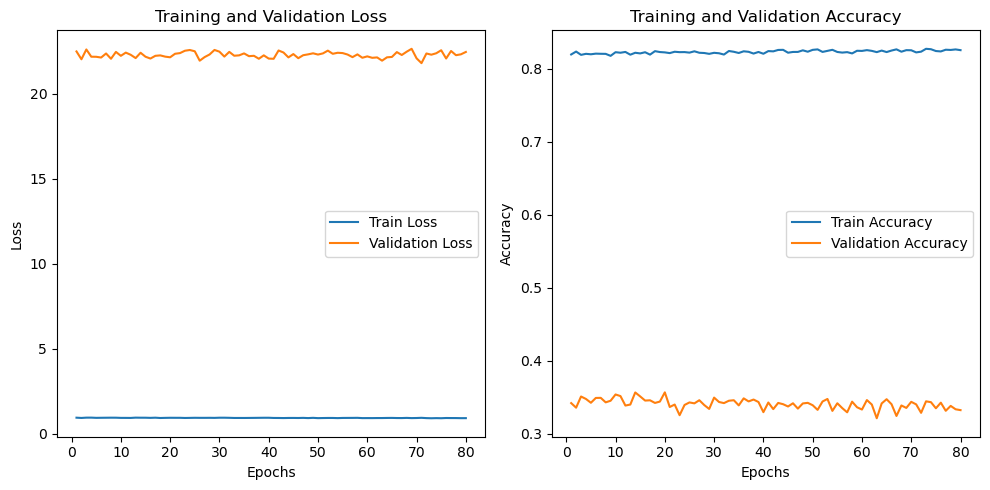
\includegraphics[width=1\linewidth]{testres.png}

\subsection{Testing results}
loss:  7.3584 - accuracy:  0.5487\\
answer-accuracy:  0.4041 - answer-type-accuracy:  0.8485

\subsection{Test samples}
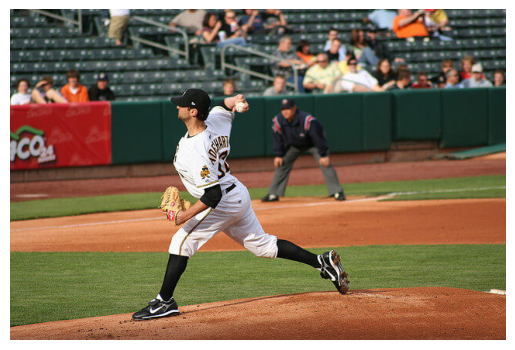
\includegraphics[width=0.5\linewidth]{baseball.png}\\
what is this?
predicted answer:unanswerable, and the type: other
\\
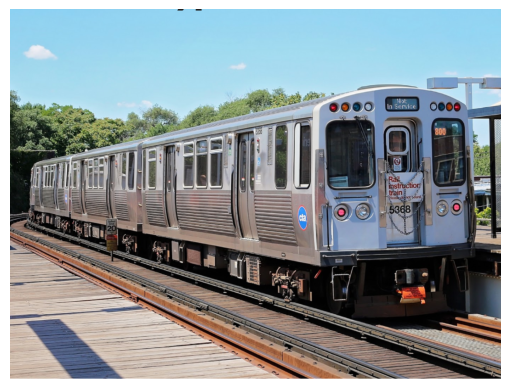
\includegraphics[width=0.5\linewidth]{train.png}\\
what is the type of this vehicle?\\
predicted answer:unanswerable, and the type: unanswerable\\
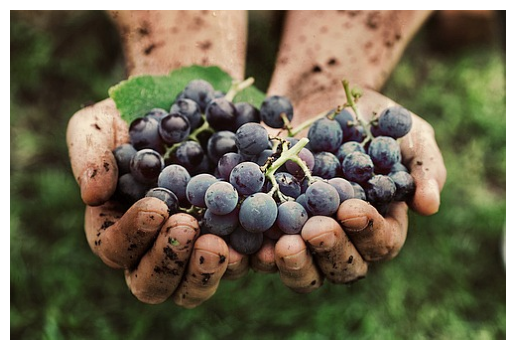
\includegraphics[width=0.5\linewidth]{grape.png}\\
what is this?\\
predicted answer:unanswerable, and the type: other\\


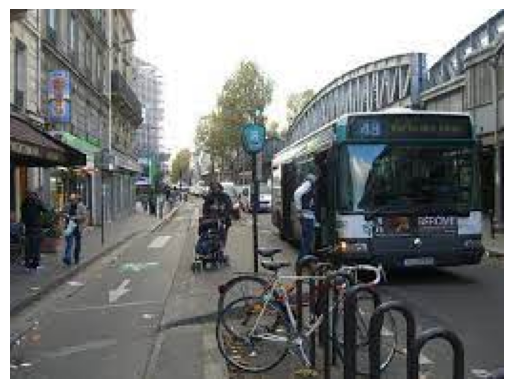
\includegraphics[width=0.5\linewidth]{bus.png}\\
    
what is this?\\
predicted answer:unanswerable, and the type: unanswerable\\


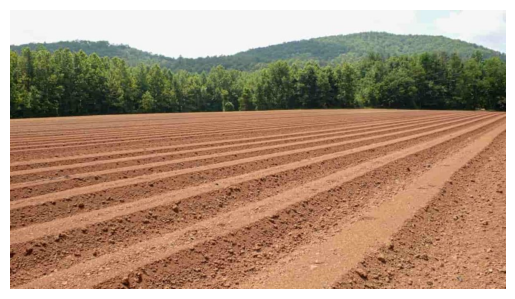
\includegraphics[width=0.5\linewidth]{land.png}\\
what is the color?\\
predicted answer:black, and the type: other




\end{document}
